\documentclass[tikz]{standalone}
\usetikzlibrary{positioning, arrows.meta, calc, fit, backgrounds}

\begin{document}
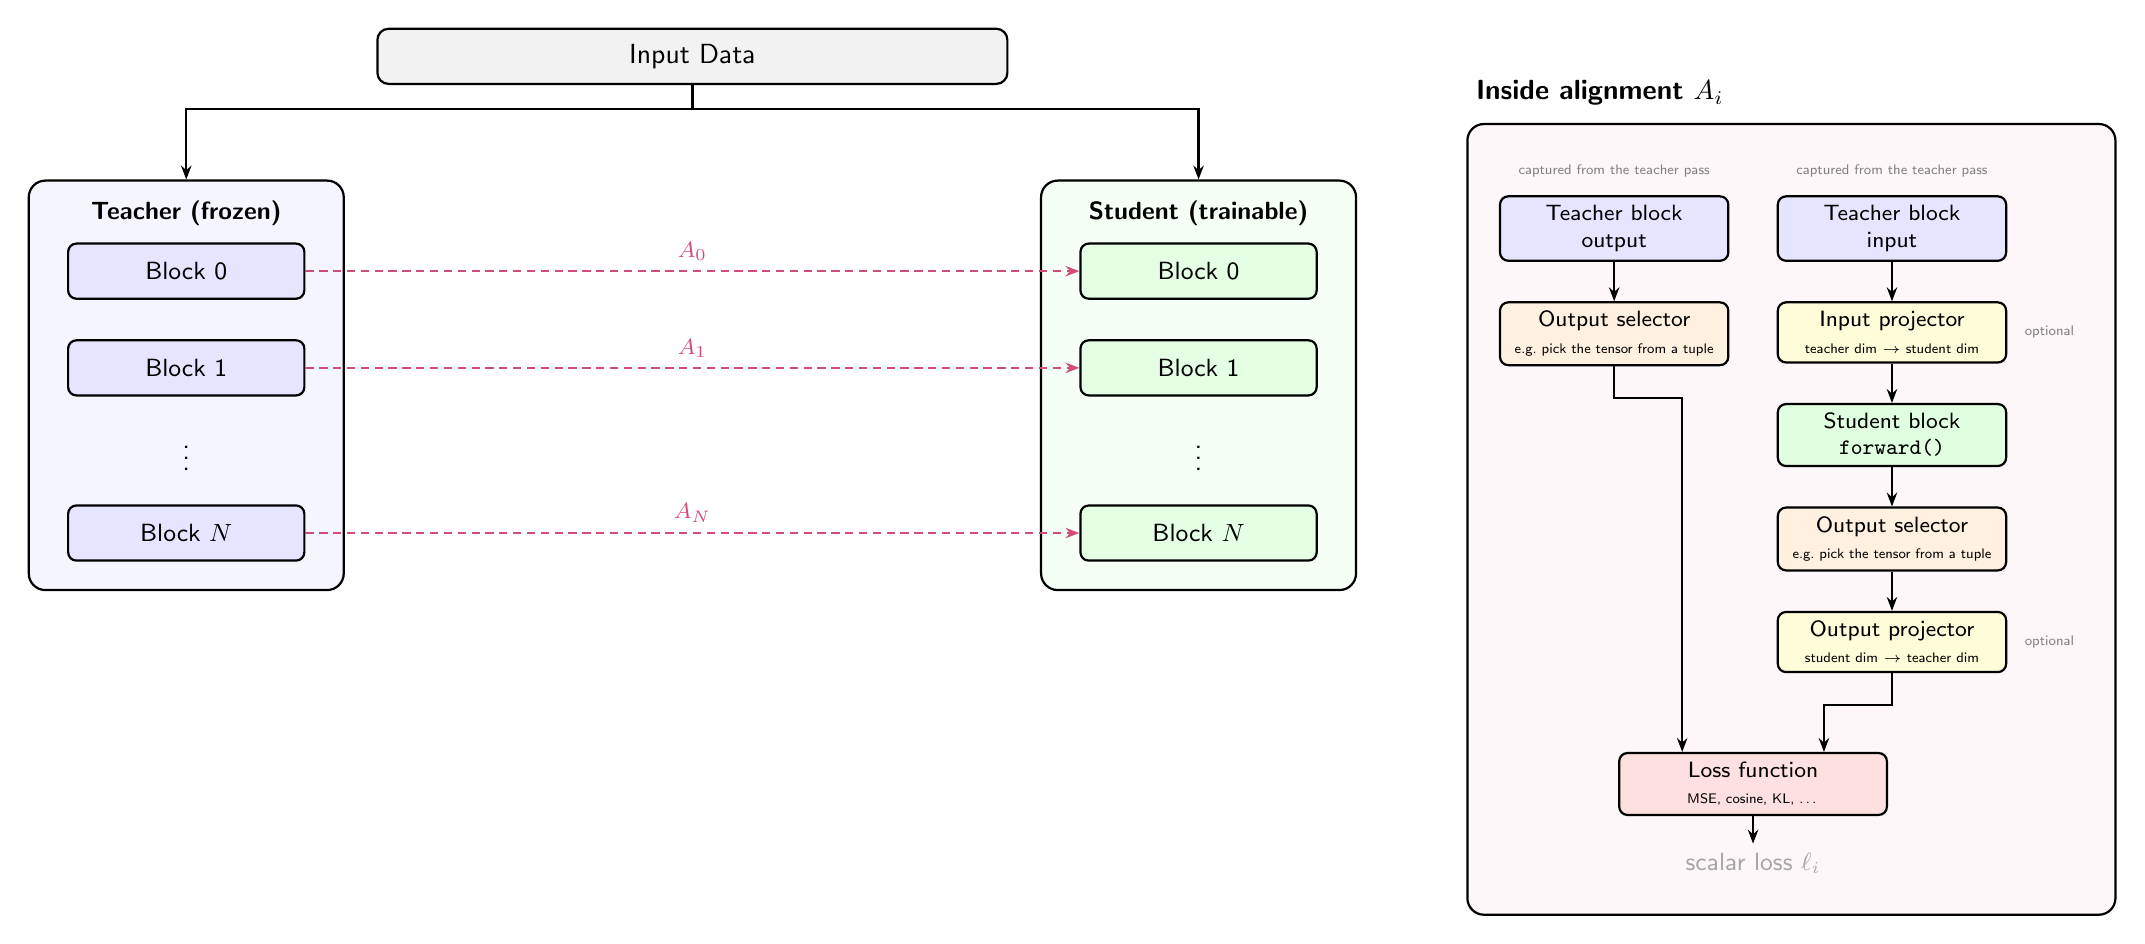
\begin{tikzpicture}[
    every node/.style={font=\sffamily},
    modelbox/.style={draw, thick, rounded corners=6pt, minimum width=4cm},
    block/.style={draw, thick, fill=#1, minimum width=3cm, minimum height=0.7cm, rounded corners=3pt, font=\sffamily\small},
    block/.default={white},
    compbox/.style={draw, thick, fill=#1, minimum width=2.9cm, minimum height=0.75cm, rounded corners=3pt, font=\sffamily\footnotesize, align=center},
    compbox/.default={white},
    note/.style={font=\sffamily\tiny, color=gray},
    arr/.style={-{Stealth[length=5pt]}, thick},
    alignarr/.style={-{Stealth[length=5pt]}, thick, densely dashed, color=purple!70},
]

% ══ Left: overview ═══════════════════════════════════════════════════════════

\node[draw, thick, rounded corners=4pt, fill=gray!10, minimum width=8cm, minimum height=0.7cm] (input) {Input Data};

\node[modelbox, fill=blue!4, below left=1.2cm and 0.4cm of input, minimum height=5.2cm] (tframe) {};
\node[font=\sffamily\bfseries\small, anchor=north] at ([yshift=-0.15cm]tframe.north) {Teacher (frozen)};

\node[modelbox, fill=green!4, below right=1.2cm and 0.4cm of input, minimum height=5.2cm] (sframe) {};
\node[font=\sffamily\bfseries\small, anchor=north] at ([yshift=-0.15cm]sframe.north) {Student (trainable)};

\node[block=blue!10, below=0.8cm of tframe.north] (tb0) {Block 0};
\node[block=blue!10, below=0.5cm of tb0] (tb1) {Block 1};
\node[below=0.3cm of tb1] (tdots) {$\vdots$};
\node[block=blue!10, below=0.3cm of tdots] (tbn) {Block $N$};

\node[block=green!10] at (tb0 -| sframe) (sb0) {Block 0};
\node[block=green!10] at (tb1 -| sframe) (sb1) {Block 1};
\node at (tdots -| sframe) (sdots) {$\vdots$};
\node[block=green!10] at (tbn -| sframe) (sbn) {Block $N$};

\draw[alignarr] (tb0.east) -- node[above, font=\sffamily\footnotesize, color=purple!70] {$A_0$} (sb0.west);
\draw[alignarr] (tb1.east) -- node[above, font=\sffamily\footnotesize, color=purple!70] {$A_1$} (sb1.west);
\draw[alignarr] (tbn.east) -- node[above, font=\sffamily\footnotesize, color=purple!70] {$A_N$} (sbn.west);

\draw[arr] (input.south) -- ++(0,-0.3) -| (tframe.north);
\draw[arr] (input.south) -- ++(0,-0.3) -| (sframe.north);

% ══ Right: inside one alignment ══════════════════════════════════════════════
% Two columns: the teacher side (what the student is compared against) and the
% student side (what is trained), meeting in the loss function.

\coordinate (panel) at ([shift={(1.8cm,-0.2cm)}]sframe.north east);

% teacher column
\node[compbox=blue!10, anchor=north west] (tout) at (panel) {Teacher block\\output};
\node[compbox=orange!12, below=0.5cm of tout] (tosel) {Output selector\\{\tiny e.g.\ pick the tensor from a tuple}};

% student column
\node[compbox=blue!10, right=0.6cm of tout] (tin) {Teacher block\\input};
\node[compbox=yellow!15, below=0.5cm of tin] (iproj) {Input projector\\{\tiny teacher dim $\to$ student dim}};
\node[compbox=green!12, below=0.5cm of iproj] (sfwd) {Student block\\\texttt{forward()}};
\node[compbox=orange!12, below=0.5cm of sfwd] (sosel) {Output selector\\{\tiny e.g.\ pick the tensor from a tuple}};
\node[compbox=yellow!15, below=0.5cm of sosel] (oproj) {Output projector\\{\tiny student dim $\to$ teacher dim}};

\node[note, anchor=west] (opt1) at ([xshift=0.1cm]iproj.east) {optional};
\node[note, anchor=west] (opt2) at ([xshift=0.1cm]oproj.east) {optional};

% loss, centred under both columns
\coordinate (lossrow) at ([yshift=-1.0cm]oproj.south);
\coordinate (midcol)  at ($(tout.center)!0.5!(tin.center)$);
\node[compbox=red!12, minimum width=3.4cm, anchor=north] (loss) at (midcol |- lossrow) {Loss function\\{\tiny MSE, cosine, KL, \ldots}};
\node[font=\sffamily\small, text=gray!70, below=0.35cm of loss] (scalar) {scalar loss $\ell_i$};

% column notes
\node[note, anchor=south, align=center] (tnote) at ([yshift=0.1cm]tout.north) {captured from the teacher pass};
\node[note, anchor=south, align=center] (snote) at ([yshift=0.1cm]tin.north)  {captured from the teacher pass};

% arrows inside the panel
\draw[arr] (tout) -- (tosel);
\draw[arr] (tosel.south) -- ++(0,-0.4) -| ([xshift=-0.9cm]loss.north);
\draw[arr] (tin) -- (iproj);
\draw[arr] (iproj) -- (sfwd);
\draw[arr] (sfwd) -- (sosel);
\draw[arr] (sosel) -- (oproj);
\draw[arr] (oproj.south) -- ++(0,-0.4) -| ([xshift=0.9cm]loss.north);
\draw[arr] (loss) -- (scalar);

% panel frame and title
\begin{pgfonlayer}{background}
    \node[draw, thick, rounded corners=6pt, fill=purple!3, inner sep=0.4cm,
          fit=(tnote)(snote)(tout)(tin)(tosel)(oproj)(opt1)(opt2)(loss)(scalar)] (abox) {};
\end{pgfonlayer}
\node[font=\sffamily\bfseries, anchor=south west] at ([yshift=0.1cm]abox.north west) {Inside alignment $A_i$};

\end{tikzpicture}
\end{document}
